\section{KI-Komponente zur automatisierten Pflanzenklassifikation}
Ziel dieses Moduls war der Aufbau eines robusten Deep-Learning-Modells zur Klassifikation von Pflanzenarten anhand fotografischer Bilddaten. Als Datengrundlage diente der PlantNet-300K-Datensatz, ein umfassender, realweltlicher Datensatz, der über 300.000 Pflanzenbilder aus verschiedenen Regionen und Perspektiven umfasst \cite{Affouard2017}. Der Ausgangsdatensatz enthielt über 1.000 Pflanzenklassen, wobei ein starker Klassenunterschied hinsichtlich der Bildanzahl pro Klasse vorlag – von 1 Bildern bis zu über 5.000 Bildern pro Art. Um ein Mindestmaß an statistischer Repräsentation zu gewährleisten und extreme Ausreißerklassen zu vermeiden, wurden für das Training ausschließlich Klassen berücksichtigt, die mindestens 5 Bilder enthielten. Diese Filterung reduzierte das Klassenspektrum auf 837 distinkte Pflanzenarten.
Diese Klassen besteht zum Großteils aus nicht sehr verbreiteten Pflanzen in Deutschland.

\subsection{Modellarchitektur und Trainingsstrategie}

Die Trainingspipeline basiert vollständig auf einem vortrainierten \ac{ResNet50}-Modell, das von Beginn an zur Initialisierung genutzt wurde. Die Wahl von \ac{ResNet50} ergibt sich aus mehreren architektonischen und empirisch belegten Vorteilen: \ac{ResNet} wurde eingeführt, um ein zentrales Problem tiefer neuronaler Netze zu adressieren – das sogenannte \emph{Degradationsproblem}. Dabei nimmt bei tiefer werdenden Netzen nicht nur die Trainingszeit zu, sondern mitunter sogar die Klassifikationsleistung ab, obwohl das Netz mehr Kapazität besitzt \cite{He2015}.

Der Kernmechanismus zur Lösung dieses Problems sind \emph{Residual-Blöcke}. Statt rohe Ausgaben direkt weiterzureichen, lernen ResNet-Blöcke nur die Abweichung von der Identität\cite{He2015}.

Das \ac{ResNet50}-Modell besteht aus insgesamt 50 Schichten, die sich aufteilen in:
\begin{itemize}
	\item eine initiale Convolution-Schicht (7x7 Convolution + MaxPooling),
	\item 16 sogenannte „Bottleneck“-Blöcke mit je drei Schichten (1x1 $\rightarrow$ 3x3 $\rightarrow$ 1x1 Convolution),
	\item Batch-Normalisierung und ReLU-Aktivierung in jedem Block,
	\item eine globale Average-Pooling-Schicht,
	\item sowie eine abschließende Fully-Connected-Schicht zur Klassifikation.
\end{itemize}

Durch diese Struktur ist \ac{ResNet50} nicht nur leistungsfähig, sondern auch besonders übertragbar auf neue Datendomänen – ein Umstand, der in einer Vielzahl an Transfer-Learning-Studien belegt wurde \cite{Kornblith2019}. Die Tiefe erlaubt es dem Modell, auch feine, visuell komplexe Unterschiede zwischen Pflanzenarten zu modellieren, während die Sprungverbindungen die Stabilität im Training erhalten.

 Im initialen Training wurden alle Schichten des Netzwerks feinjustiert. Nach einer ersten Konvergenz wurde ein Finetuning durchgeführt, bei dem ein Großteil der Layer eingefroren wurde, um ausschließlich die letzten Klassifikationsschichten anzupassen. Dieses zweistufige Vorgehen ist ein gängiger Transfer-Learning-Ansatz, insbesondere wenn ein großes Ausgangsmodell (wie \ac{ResNet}) auf eine domänenspezifische Aufgabe adaptiert wird \cite{Pan2010}.

\subsection{Regularisierung und Datenkonsolidierung}
Zur Verbesserung der Modellrobustheit wurden mehrere datenaugmentierende Verfahren eingesetzt. Dazu zählen insbesondere Mixup \cite{Zhang2018} und CutMix \cite{Yun2019}, welche zu besseren Verallgemeinerungseigenschaften führen, indem sie die Entscheidungsgrenzen im Merkmalsraum glätten. Ergänzt wurden diese Verfahren durch RandAugment, eine robuste Augmentierungsmethode ohne komplexe Hyperparametrierung.

Ein zentrales Vorverarbeitungsschritt war die Anwendung des Moduls \file{create\_merge\_map.py}, das vor dem Finetuning genutzt wurde, um Duplikate und taxonomisch redundante Pflanzenklassen zusammenzuführen. Diese Maßnahme reduziert das Risiko semantischer Verwirrung im Trainingsprozess und wurde insbesondere bei identischen oder sehr ähnlichen Arten eingesetzt. Die Notwendigkeit solcher Label-Konsolidierungen ist insbesondere in crowd-basierten, multilinguistisch annotierten Datensätzen wie PlantNet belegt \cite{Horn2018}.

Darüber hinaus wurde zur Kompensation des hochgradig unausgeglichenen Klassenverhältnisses (5–5000 Bilder pro Klasse) ein Weighted Sampling implementiert. Diese Technik erhöht die Wahrscheinlichkeit der Auswahl von Bildern seltener Klassen während des Batch-Trainings und verhindert so die Dominanz überrepräsentierter Arten im Gradientenfluss – ein gängiger Ansatz zur Balancierung von Imbalancen in Klassifikationsaufgaben \cite{Buda2018}.

\subsection{Leistung und Interpretation}

Die Trainingszeit betrug insgesamt 65 Stunden, wobei 50 Stunden auf das initiale, vollständig entfrorene Training und 15 Stunden auf das anschließende Finetuning entfielen.

Das finale Modell demonstrierte eine hohe Klassifikationsfähigkeiten. Die Top-1-Accuracy von 77\% bedeutet, dass das Modell in über drei Viertel aller Fälle die exakte Pflanzenart korrekt identifizierte. Die Top-5-Accuracy von 95\% zeigt, dass sich die wahre Klasse in der Mehrheit der Fälle unter den fünf wahrscheinlichsten Vorhersagen befand – ein Maß, das insbesondere in praktischen Anwendungen wie botanischen Bestimmungs-Apps von Relevanz ist. In der Abbildung \vref{fig:plantAI} sind Beispiel zu sehen.

\begin{figure}[H]
	\centering
	
	% Erste Zeile
	\begin{minipage}[t]{0.40\textwidth}
		\centering
		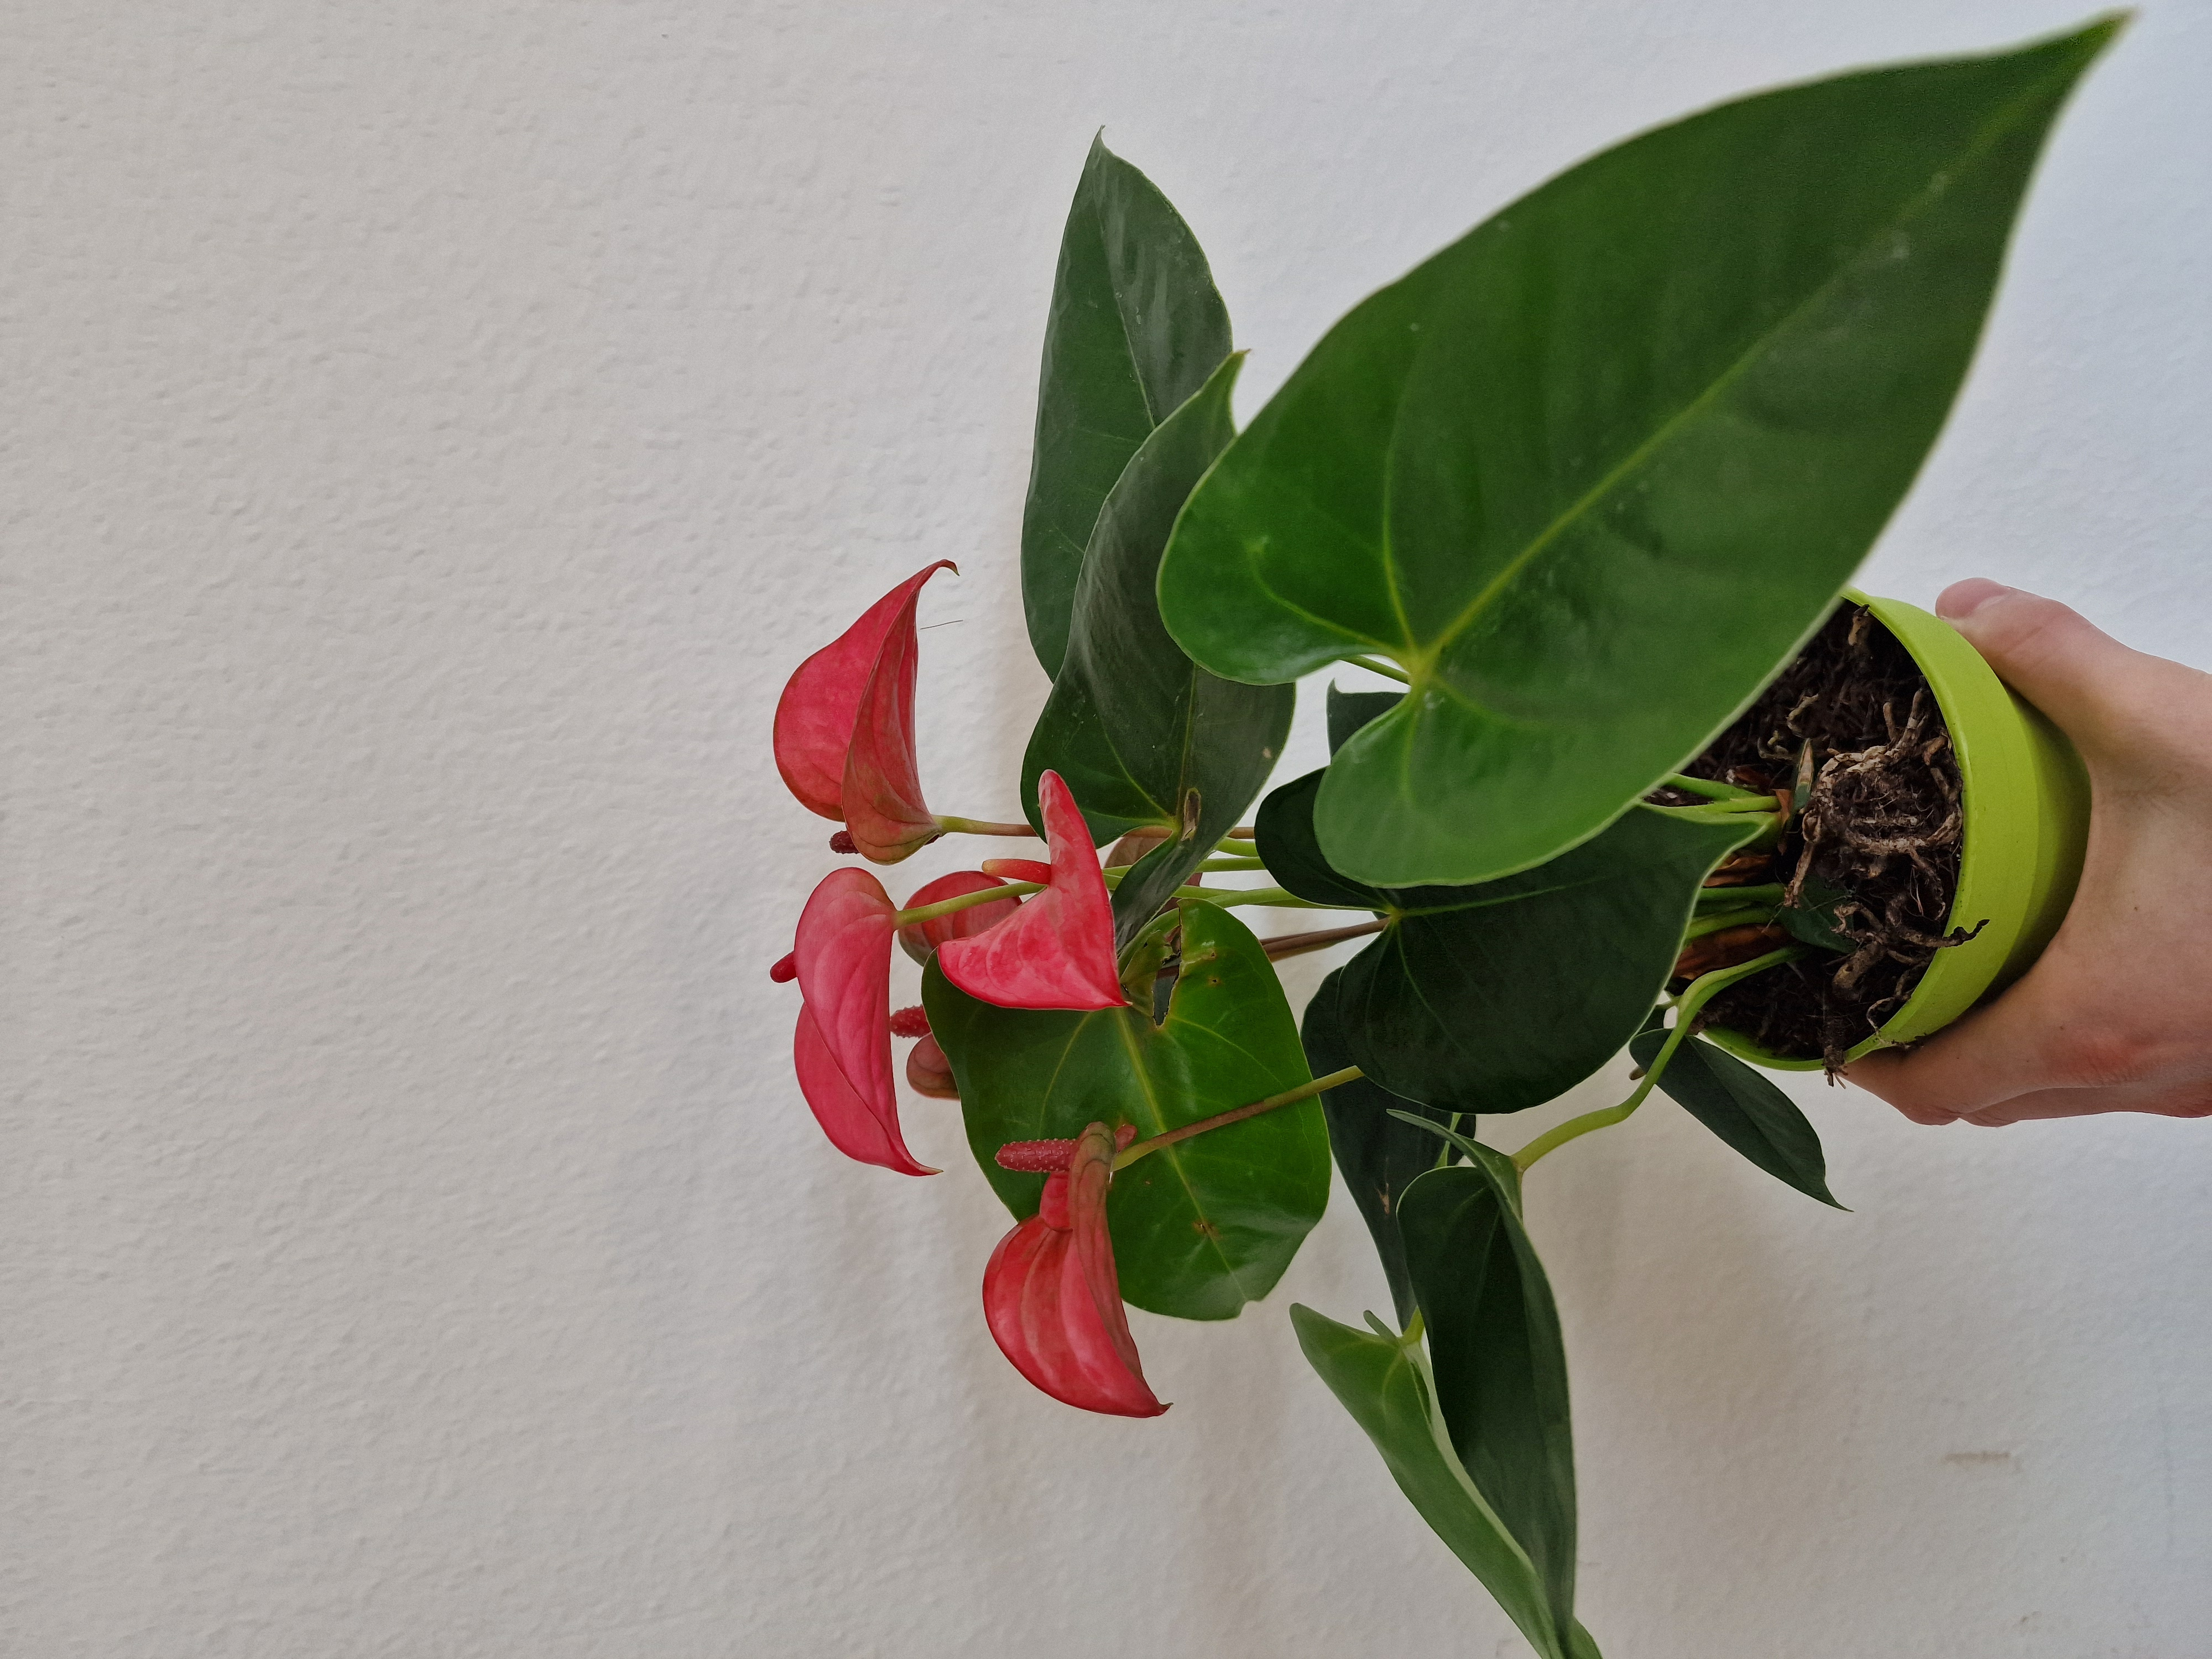
\includegraphics[angle=-90, width=\linewidth]{./Umsetzung/images/1.jpg}
		\caption{Korrekt erkannt als Anthurium Andraeanum mit 99,72\%}
	\end{minipage}
	\hfill
	\begin{minipage}[t]{0.40\textwidth}
		\centering
		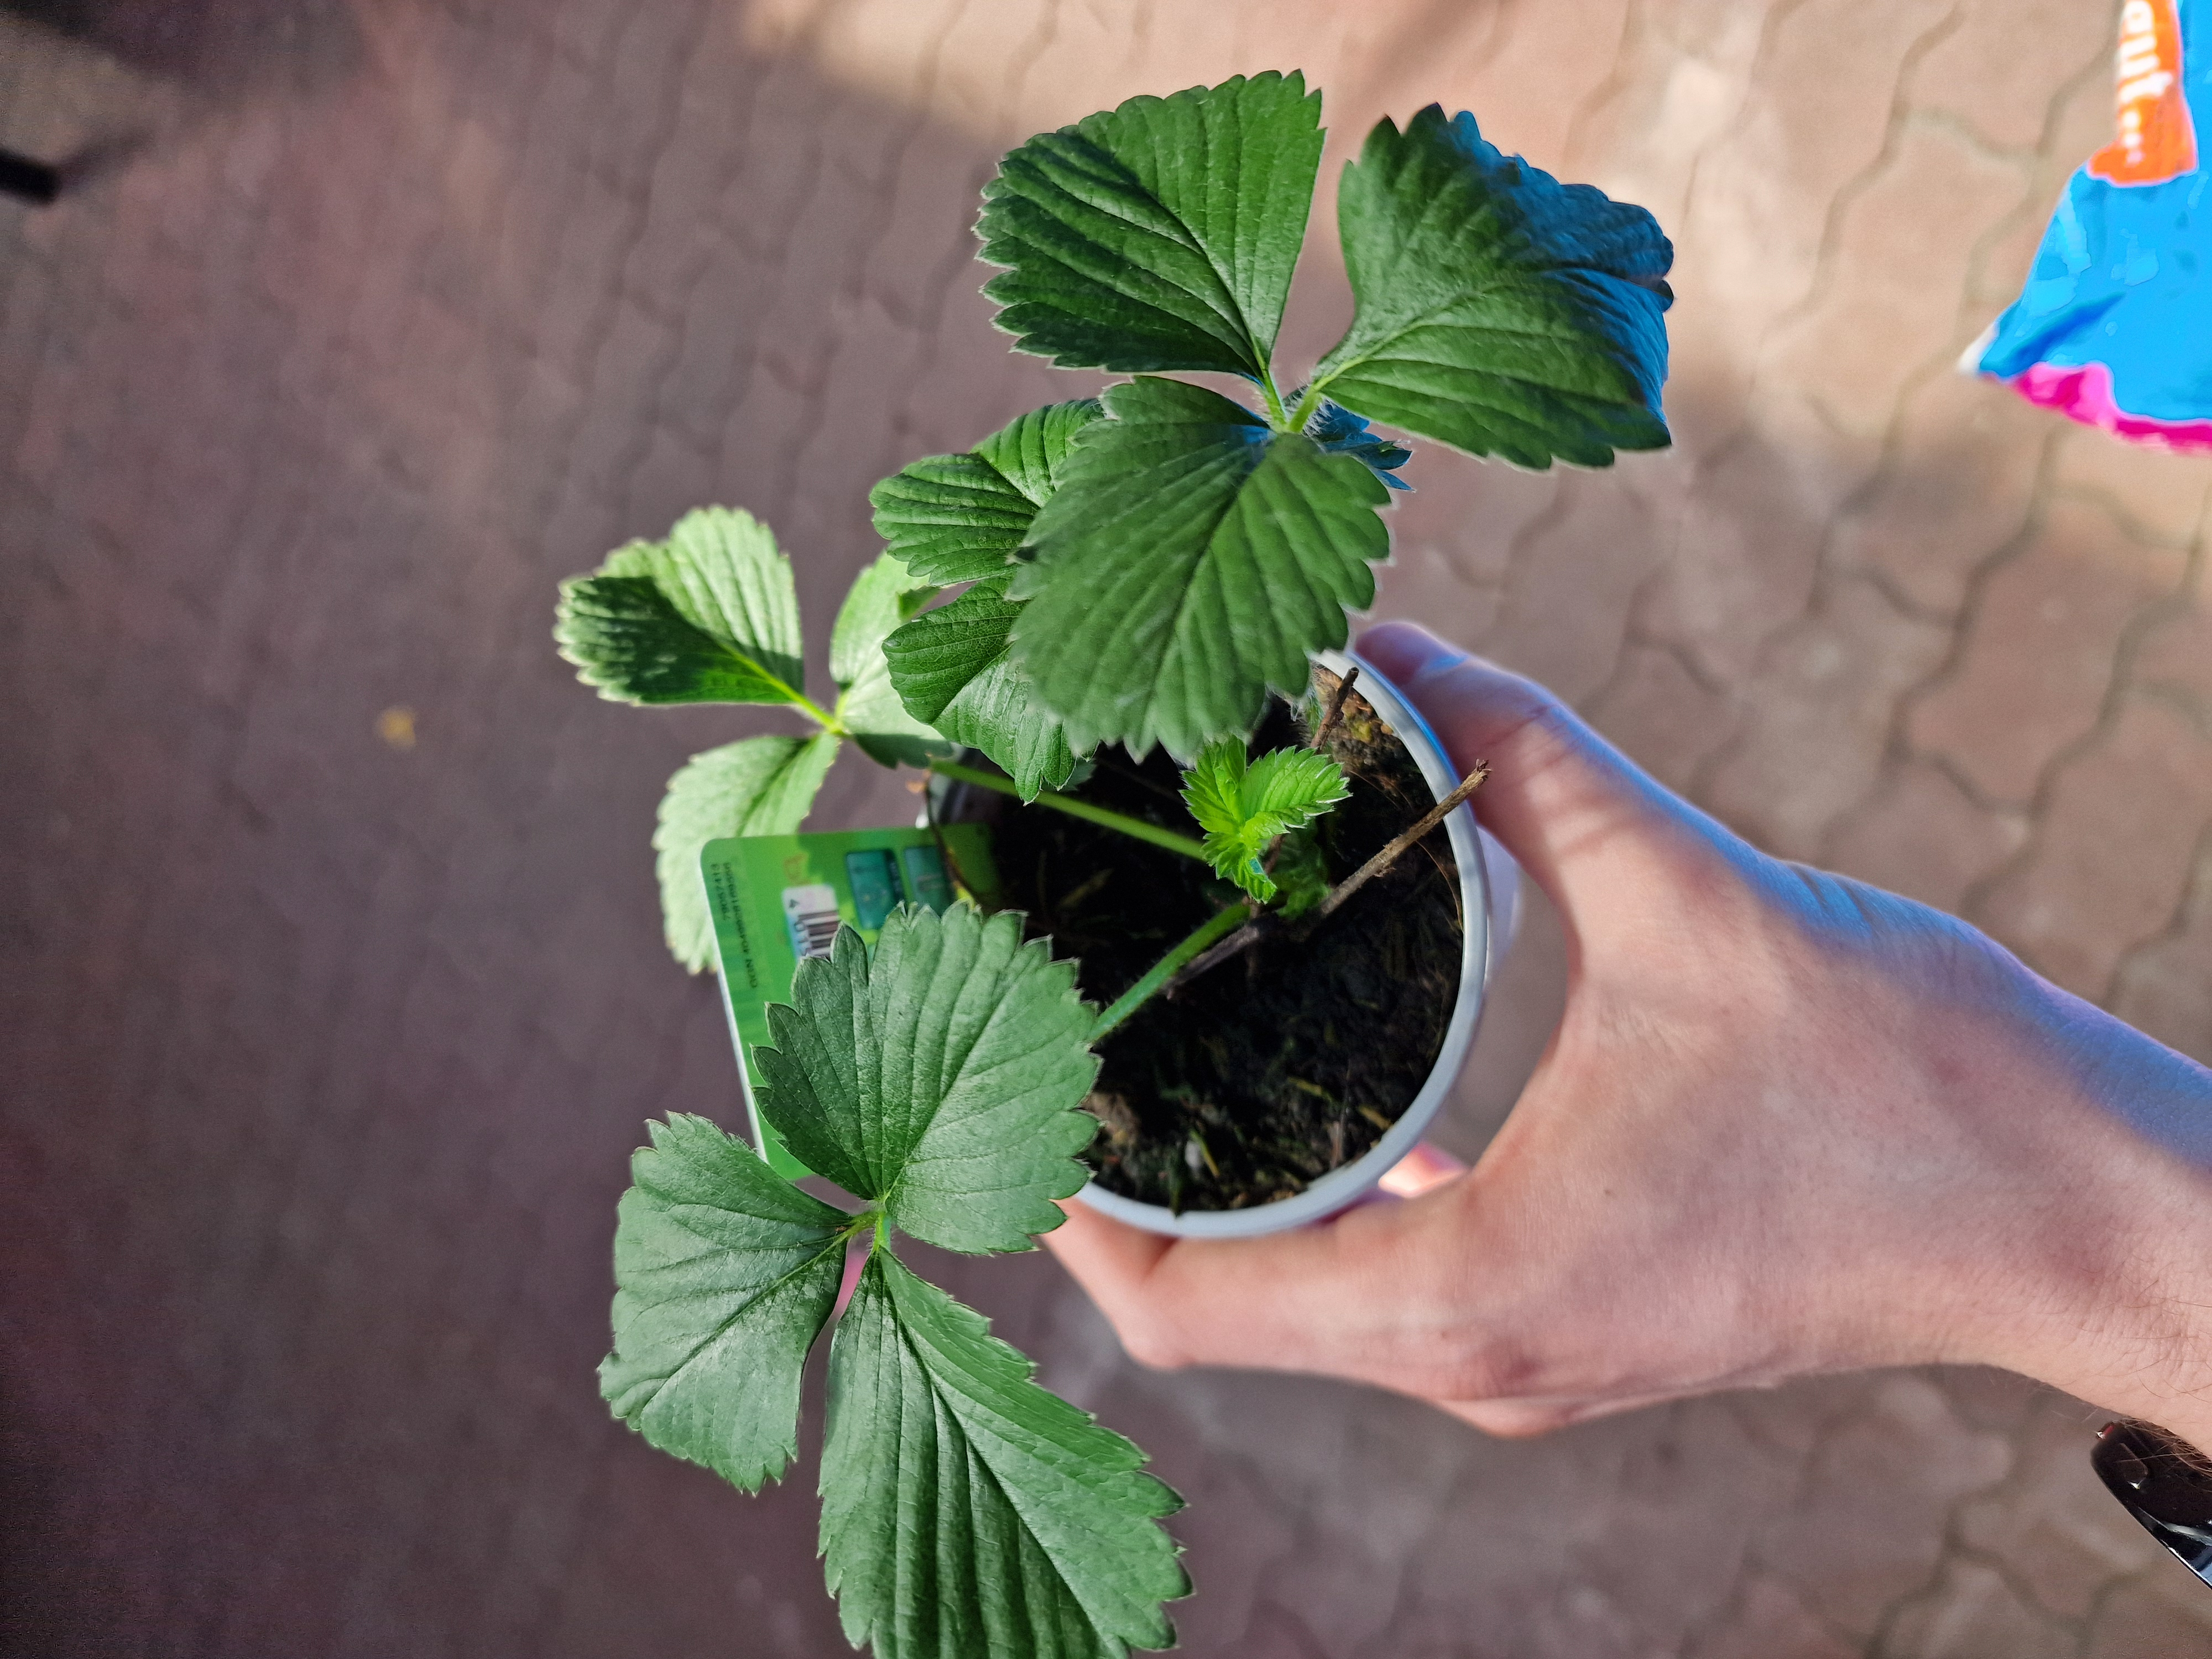
\includegraphics[angle=-90, width=\linewidth]{./Umsetzung/images/2.jpg}
		\caption{Korrekt erkannt als Fragaria X Ananassa mit 90,42\%}
	\end{minipage}
	
	\vspace{0.3em}
	\begin{minipage}{\textwidth}
		\centering
		\small Abbildung oben: Übersicht einiger markanter Testpflanzen.
	\end{minipage}
	
	\vspace{1em}
	
	% Zweite Zeile
	\begin{minipage}[t]{0.40\textwidth}
		\centering
		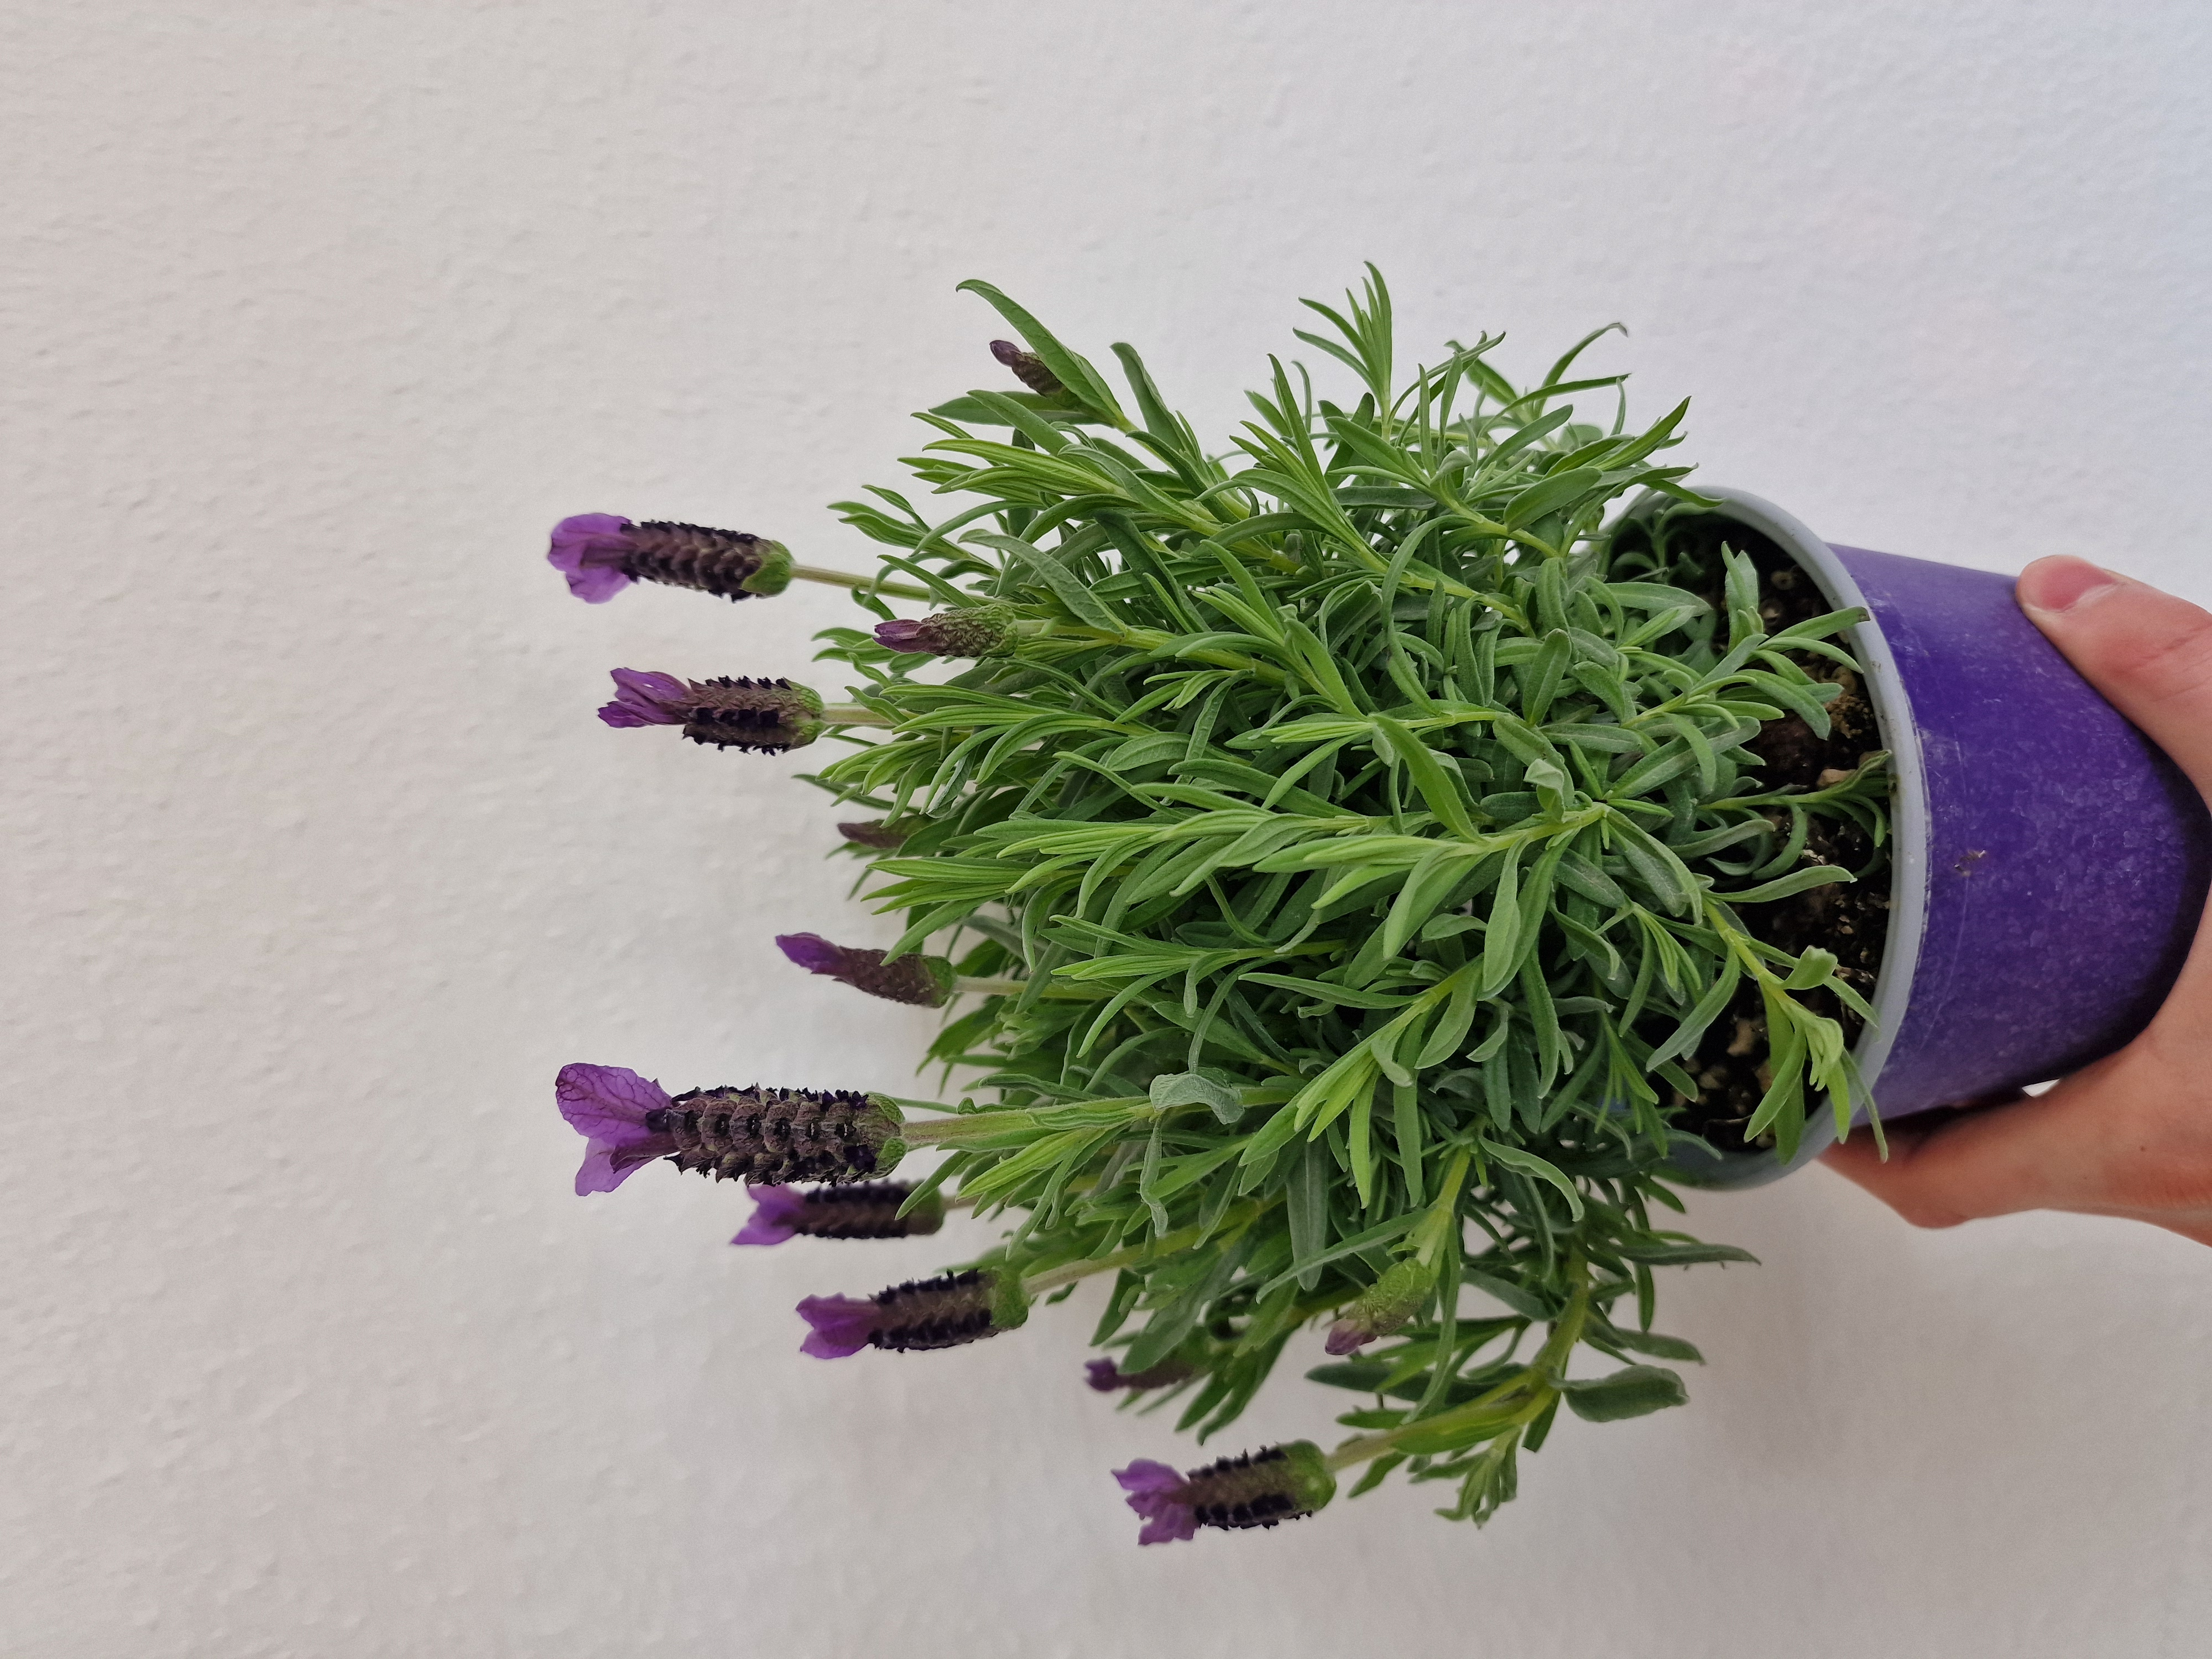
\includegraphics[angle=-90, width=\linewidth]{./Umsetzung/images/3.jpg}
		\caption{Korrekt erkannt als Lavandula Stoechas mit 99,49\%}
	\end{minipage}
	\hfill
	\begin{minipage}[t]{0.40\textwidth}
		\centering
		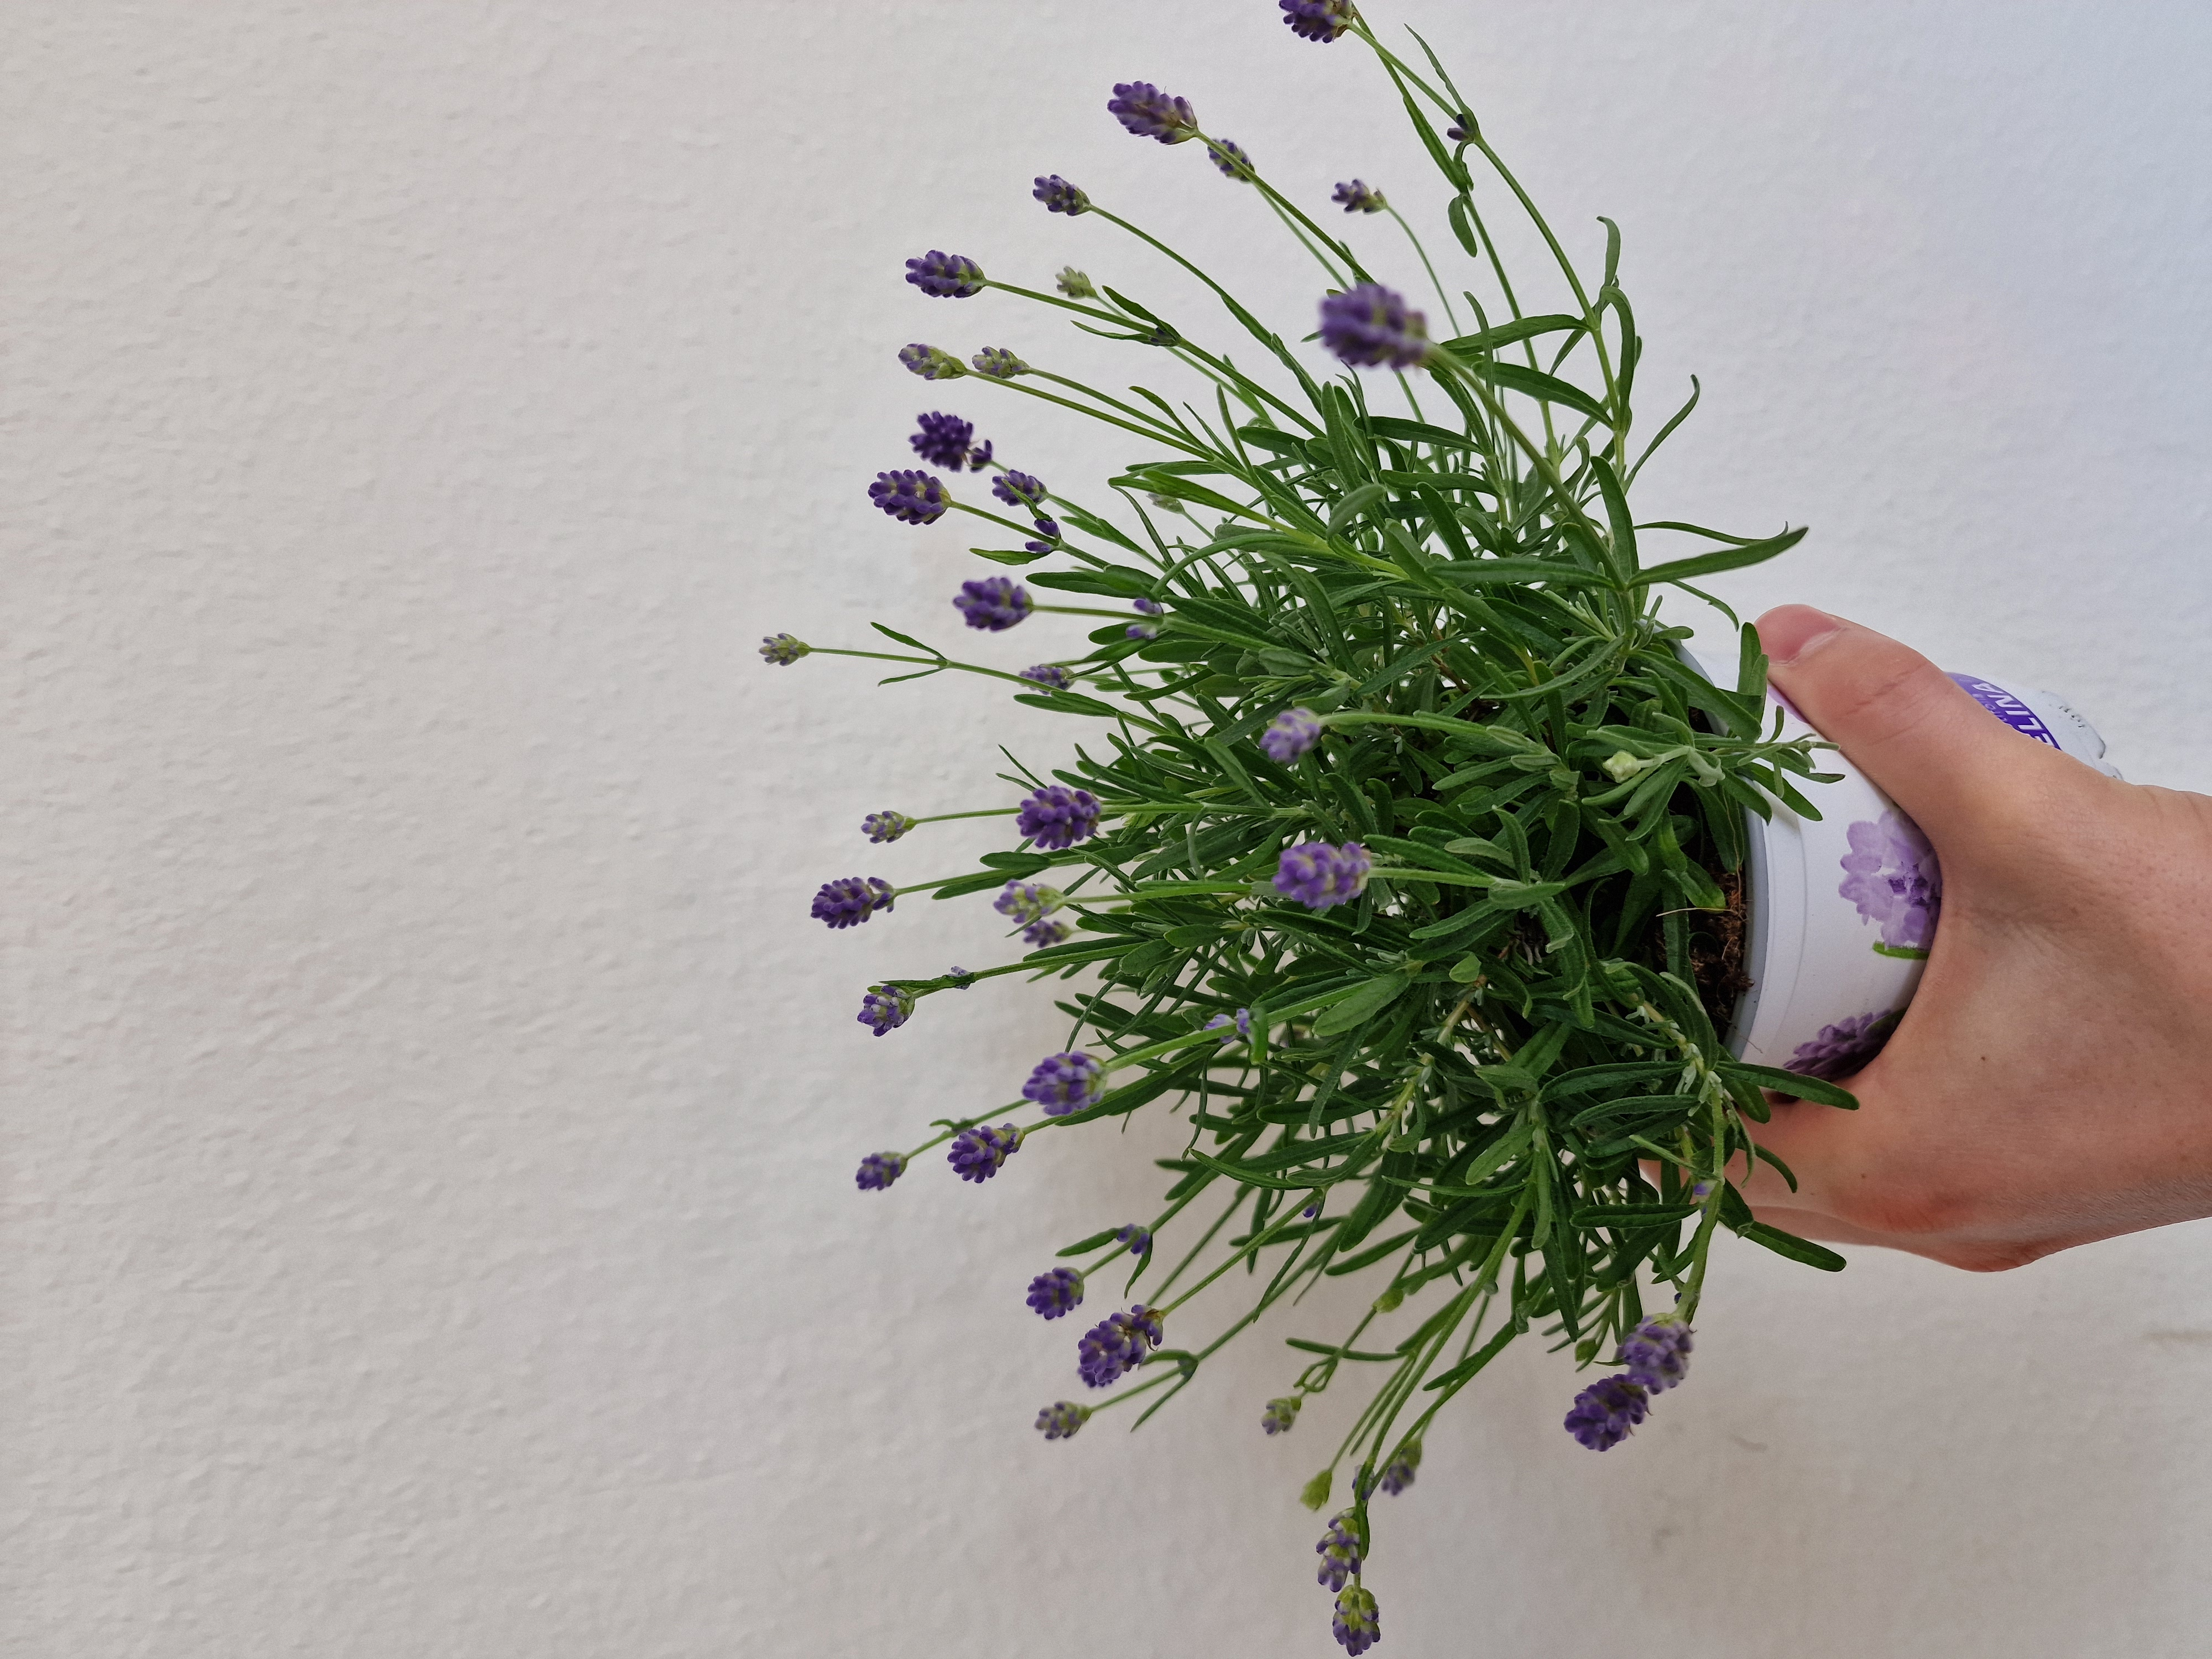
\includegraphics[angle=-90, width=\linewidth]{./Umsetzung/images/4.jpg}
		\caption{Korrekt erkannt als Lavandula Angustifolia mit 98,05\%}
	\end{minipage}
	
	\vspace{0.3em}
	\begin{minipage}{\textwidth}
		\centering
		\small Abbildung unten: Vergleich der Genauigkeit zweier Lavendel Arten
	\end{minipage}
	
	\caption{Beispiel für die KI-Erkennung}
	\label{fig:plantAI}
\end{figure}



\subsection{Rolle der KI-Komponente bei der Pflanzenerstellung}

Die KI-Komponente wird im Gesamtsystem insbesondere bei der Erstellung neuer Pflanzeninstanzen eingesetzt. NutzerInnen haben dabei die Möglichkeit, grundlegende Eigenschaften einer Pflanze – wie den Pflanzennamen oder die Artzugehörigkeit – automatisiert durch ein KI-Modul bestimmen zu lassen. Dieser Vorgang kann sowohl durch das Hochladen eines bestehenden Pflanzenbilds als auch direkt über eine Fotoaufnahme im Browser oder auf mobilen Endgeräten ausgelöst werden. Alternativ besteht die Möglichkeit, ohne KI-Unterstützung nach einer Pflanze zu suchen.

Bei Nutzung der KI-Komponente wird das Bild über das Frontend an einen dedizierten Klassifikationsservice übermittelt. Dieser führt eine Inferenz mit dem trainierten \ac{ResNet50}-Modell durch und schlägt basierend auf der Bildanalyse eine Pflanzenart vor. Neben der wahrscheinlichsten Klasse wird zusätzlich eine Liste mit weiteren möglichen Arten inklusive Vorhersagewahrscheinlichkeiten generiert. Es werden aber nur Pflanzen mit über 50\% zurückgegeben. Diese Vorhersage wird visuell im Interface dargestellt und kann von der NutzerIn  bestätigt werden.

Der ausgewählte Vorschlag bildet dann die Grundlage für die Vorbelegung der Eingabefelder zur Pflanzenerstellung, sodass beispielsweise der wissenschaftliche Name, die Spezies und Soll-Werte geschätzt werden. Die KI-Komponente unterstützt somit aktiv die Datenerfassung und sorgt für eine beschleunigte, komfortable Erstellung von Pflanzendatensätzen innerhalb des Systems. Die finale Entscheidung über die Auswahl der vorgeschlagenen Pflanze verbleibt stets bei den Nutzenden.

